\section{Preliminaries}
\label{section: GraphRAG}


\subsection{Problem Formalization}

GraphRAG is designed to integrate structured knowledge into the reasoning process of LLMs, enhancing their ability to generate content that is both accurate and contextually relevant.
%appropriate content generation.
In GraphRAG, knowledge is typically represented in the form of Text-Attributed Graphs (TAGs), where both nodes and edges are enriched with textual information, with knowledge graphs serving as a typical example.
For clarity and without loss of generality, the graphs referred to in this paper will follow the structure outlined in Definition~\ref{def:graph}.


\begin{definition}[{\bf Graph in GraphRAG}]
	\label{def:graph}
In GraphRAG, a graph is defined as a directed labeled graph \( G = (V, E) \), where \( V \) represents the set of nodes (entities), and \( E \) denotes the set of directed edges that signify relations between those entities. Each node \( v \in V \) and each edge \( e \in E \) carry semantic information. Specifically, nodes represent entities with associated semantic attributes (e.g., descriptions), while edges represent relations with semantic contexts (e.g., relation types). 

Formally, the graph in GraphRAG is represented as a collection of triples: $G = \{ \tau_i = (s_i, r_i, t_i) \mid s_i, t_i \in V, r_i \in E \}$ , 
%\begin{equation}
%\small G = \{ \tau_i = (s_i, r_i, t_i) \mid s_i, t_i \in V, r_i \in E \} \end{equation}
where each \( \tau_i = (s_i, r_i, t_i) \) is a triple representing that the source entity \( s_i \) is connected to the target entity \( t_i \) by the relation \( r_i \), encapsulating structured, domain-specific knowledge. While a single triple \( \tau_i \) is a basic unit of knowledge, a sequence of connected triples forms reasoning paths that support more advanced inferences.
\end{definition}


In practice, graphs are built from domain knowledge
or text (e.g., Microsoft GraphRAG~\cite{GraphRAG} with auxiliary summaries; see Definition~\ref{def:graph_con}). As text-to-graph construction is well-studied~\cite{GraphRAG,LightRAG,KAG,ref:hipporag,sac-kg} and not central to our framework, we treat it as optional but include a GraphRAG instance with textual information in our analysis (Section~\ref{exp:instance} e).
%In practice, graphs are either pre-constructed using domain knowledge or obtained from structured knowledge sources. Following Microsoft GraphRAG, graphs can also be constructed from text, with auxiliary precomputed textual information, as defined in Definition~\ref{def:graph_con}. 
%Since text-to-graph construction has been extensively studied and is not the focus of our framework, we consider it optional.
%As a complement, we include the Microsoft GraphRAG instance with auxiliary  textual information in our empirical analysis in Section~\ref{exp:instance} e).



\begin{definition}[{\bf Graph Construction ({\it Optional})}]
\label{def:graph_con}
In GraphRAG, graph construction is an optional step that builds a text-attributed graph from large-scale text,  and may also precompute subgraphs and summaries to enhance GraphRAG.
Specifically:
\begin{itemize}[leftmargin=10pt]
    \item \textbf{Construction:} Identify entities and relations from text and represent them as nodes and edges in the graph.

    \item \textbf{Precomputation ({\it Optional}):} Compute subgraphs and relevant textual summaries from the constructed graph, such as via graph clustering or community detection. 
\end{itemize}
\end{definition}


    
%Here is a specific example of a graph:
\begin{comment}

\begin{tcolorbox}[breakable, colframe=black, colback=black!5!white!50, boxrule=0.4mm, rounded corners, arc=0mm, left=0mm, right=0mm, top=0mm, bottom=0mm, opacityback=0.9]    \small
	\begin{example} [{\bf Graph in GraphRAG}] 	
		\label{exm:graph}
		Consider a toy graph $G=(V,E)$ that represents notable database researchers who have won the ACM Turing Award and their key contributions to the databases field. Here, $V = \{\text{Michael Stonebraker}, \text{Edgar F. Codd}, \text{Jim Gray}, \text{PostgreSQL},\\ \text{Relational Model}, \text{Transaction Processing}, \text{ACM Turing Award}\}$ represent the entities, and $E$ denotes the relations between them. The graph $G$ can be represented by the following set of triples.
		\begin{equation*}    \small
			\begin{aligned}
				G = \{ & (\text{PostgreSQL}, \text{was created}, \text{Michael Stonebraker}), \\  
				& (\text{Michael Stonebraker}, \text{awarded}, \text{ACM Turing Award}), \\  
				& (\text{Relational Model}, \text{was developed}, \text{Edgar F. Codd}), \\  
				& (\text{Edgar F. Codd}, \text{awarded}, \text{ACM Turing Award}), \\  
				& (\text{Transaction Processing}, \text{was pioneered}, \text{Jim Gray}), \\  
				& (\text{Jim Gray}, \text{awarded}, \text{ACM Turing Award}) \}
			\end{aligned}
		\end{equation*}
	\end{example}
\end{tcolorbox}
    
\end{comment}



With text-attributed auxiliary graphs, GraphRAG operates in two main phases: \textit{retrieval} and \textit{augmented generation} phases. During the retrieval phase (Definition~\ref{def:retrieval}), the system extracts relevant entities and reasoning paths from the graph, aligning them with the query context.
%are extracted from the graph. 
In the augmented generation phase (Definition~\ref{def:generation}), these retrieved reasoning paths are incorporated to enhance LLM's content generation capabilities.



\begin{definition}[{\bf  Retrieval Phase}]
	\label{def:retrieval}
This phase starts by processing the query $q$ to extract relevant entities and relations that correspond to nodes and edges in the graph $G$: $\textit{Extract} (q, G) \rightarrow \epsilon_q=(\{v_i^{(q)}\}, \{e_i^{(q)}\})$, 
%\begin{align}
%\small
%\label{eqn:extract}
%	\textit{Extract} (q, G) \rightarrow \epsilon_q=(\{v_i^{(q)}\}, \{e_i^{(q)}\})
%\end{align}
where $\epsilon_q$ is the set of entities and relations extracted.\footnote{ Extracting entities/relations from the semantic context of $q$ has been well-studied~\cite{NSM, EmbedKGQA, StructGPT} and is beyond the scope of this paper.
Following prior works on reasoning tasks in graphs~\cite{UHop,berant-etal-2013-semantic,yih-etal-2014-semantic,complex2simple,EmbedKGQA}, queries are typically categorized by the minimum number of reasoning hops required to reach the answer from the query entities or relations (e.g., one-hop queries or multi-hop queries). 
%with two or more hops
In addition, queries can also be categorized by the number of answers and the number of query entities involved. 
}

Using the extracted entities $\{v_i^{(q)}\}$ and relations $\{e_i^{(q)}\}$ in $\epsilon_q$, a variety of methods (e.g., search algorithms, neural network-based retrieval/ranking models) are applied to retrieve reasoning paths $ \mathcal{P}_q$ 
that connect $\epsilon_q$ to potential target answers, potentially spanning multiple hops.
The retrieval process is thus formalized by: $\textit{Retrieve} (\epsilon_q, G) \rightarrow \mathcal{P}_q=\{P_i^{(q)}\}$
%\begin{equation}
%\small
%	\textit{Retrieve} (\epsilon_q, G) \rightarrow \mathcal{P}_q=\{P_i^{(q)}\}
%\end{equation}
where each reasoning path $P_i^{(q)}\in \mathcal{P}_q$ of length $k$ is represented as a sequence of triples $\langle \tau_1, \tau_2, \ldots, \tau_k \rangle$: 
\begin{align*}
\small
P_i^{(q)} = \langle \tau_1, \tau_2, \ldots, \tau_k \rangle=\langle (s_1, r_1, t_1), (t_1, r_2, t_2), \ldots, (t_{k-1}, r_k, t_k) \rangle %, \quad t_j = s_{j+1}, \ \forall j
\end{align*}

\end{definition}

\begin{comment}
    

    
\begin{tcolorbox}[colframe=black, colback=black!5!white!50, boxrule=0.4mm, rounded corners, arc=0mm, left=0mm, right=0mm, top=0mm, bottom=0mm, opacityback=0.93]    \small
	\begin{example} [{\bf Retrieval}] 	
		\label{exm:retrieval}
		For the query ``{\it Who received the Turing Award for developing the Relational Model}?'', the retrieval phase begins by extracting the relevant entities and relations from the graph. 
Here, the query refers to the entities ``Relational Model'', ``ACM Turing Award'', and the relation ``was developed''. The reasoning path pertinent to the query is then retrieved.% from the graph:
		\begin{tcolorbox}[colframe=black, colback=black!5!white!50, boxrule=0.2mm, rounded corners, arc=0mm, left=0mm, right=0mm, top=0mm, bottom=0mm, opacityback=0.95, boxsep=0mm, valign=center] \small
			\begin{center}
				\footnotesize Relational Model $\xrightarrow{\text{developed by}}$ Edgar F. Codd $\xrightarrow{\text{awarded}}$ ACM Turing Award
			\end{center}
		\end{tcolorbox}
	\end{example}
\end{tcolorbox}

\end{comment}


\begin{definition}[{\bf Augmented Generation Phase}]
	\label{def:generation}
In this phase, the retrieved reasoning paths $\mathcal{P}_q$ are merged with the original query $q$, forming an augmented prompt $q'$: $\textit{Augment}(q, \mathcal{P}_{q}) \rightarrow q'$.
%\begin{equation}
%    \small
%	\textit{Augment}(q, \mathcal{P}_{q}) \rightarrow q'
%\end{equation}
This augmented prompt is then input to the LLMs, enhancing their ability to generate more accurate and contextually relevant content for the final answer: $	\textit{Generate}(q', \text{LLM}) \rightarrow \textit{final answer}$.
%	\begin{equation}
%    \small
%		\textit{Generate}(q', \text{LLM}) \rightarrow \textit{final answer}
%	\end{equation}
\end{definition}

\begin{comment}
    

    
\begin{tcolorbox}[colframe=black, colback=black!5!white!50, boxrule=0.4mm, rounded corners, arc=0mm, left=0mm, right=0mm, top=0mm, bottom=0mm, opacityback=0.93]    \small
	\begin{example} [{\bf Augmentation}] 	
		\label{exm:generation}
	In the phase, the retrieved reasoning path is integrated with the original query to construct a more informative prompt for the LLMs. For example, the resulting augmented prompt used as inputs to the LLMs for generating the final answer could be:
\begin{tcolorbox}[colframe=black, colback=black!5!white!50, boxrule=0.2mm, rounded corners, arc=0mm, left=0mm, right=0mm, top=0mm, bottom=0mm, opacityback=0.95, boxsep=0mm, valign=center] \small
	Your task is to analyze the given reasoning paths and provide clear answers to the questions based on these paths.
	
	Reasoning Paths: {\it \{Relational Model, was developed, Edgar F. Codd, awarded, ACM Turing Award\}}
	
	Question: {\it \{Who received the Turing Award for developing the Relational Model?\}}
	\end{tcolorbox}
%This augmented prompt is then passed to the LLMs to generate the final answer.
	\end{example}
\end{tcolorbox}
\end{comment}

Figure~\ref{GraphRAG} illustrates the GraphRAG workflow, where retrieval forms the foundation by supplying key reasoning paths for LLM augmentation and generation. As these stages hinge on retrieval quality and LLM strength, this work focuses on analyzing the modular design and solution space of the retrieval phase.

%The workflow of GraphRAG is shown in Figure~\ref{GraphRAG}. Notably, the retrieval phase serves as the foundation of GraphRAG, delivering critical reasoning information that fuels subsequent augmentation and generation stages for LLMs. Since the augmentation and generation largely depend on the retrieved reasoning paths and the inherent strength of LLMs, this work focuses on the retrieval phase. Thus, the objective of this work is to comprehensively analyze its modular design and investigate the corresponding solution space.
%for the retrieval phase.



\begin{figure}[t]
    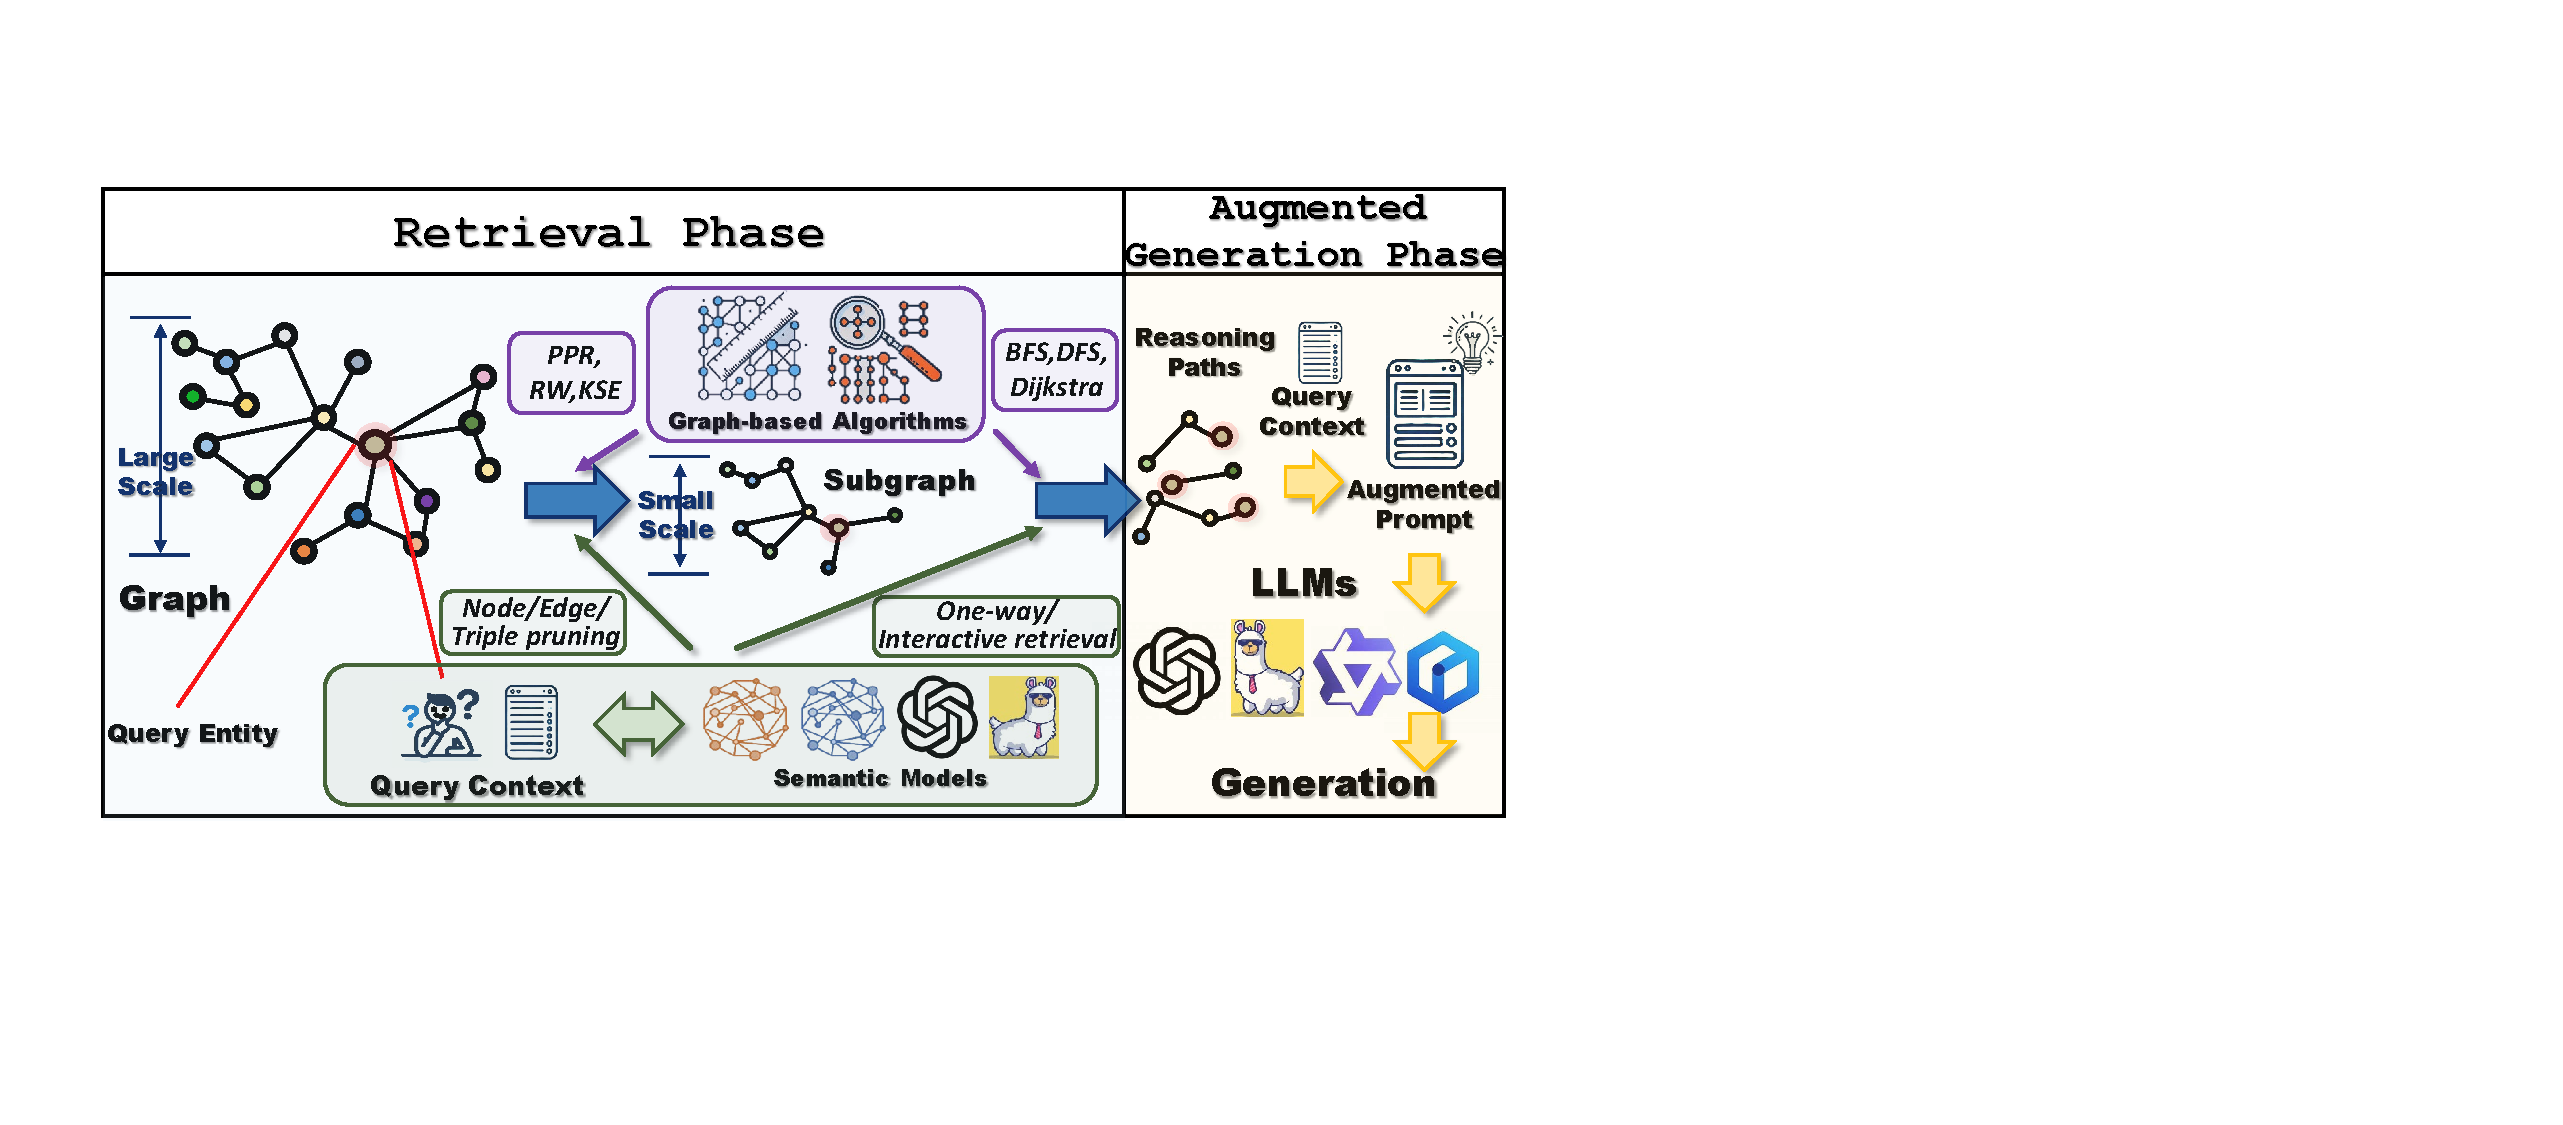
\includegraphics[width=0.98\linewidth]{figures/paper/LEGO.pdf}
    \vspace{-5pt}
    \caption{The GraphRAG Workflow} 
    \label{GraphRAG}
\end{figure}
